\documentclass{beamer}
\usepackage{amsmath, amssymb}
\usepackage{bm}
\usepackage{luatexja}
\usepackage{mathrsfs}              % 花文字
\usepackage{multirow}              % 表結合
\usepackage{float}                 % 図の位置制御
\usepackage{url}                   % URL表示
\usepackage{type1cm}               % フォント調整
\usepackage{here}                  % H位置指定
\usepackage{physics}               % 量子力学向け記法
\usepackage{graphicx}
\title{HF軌道をもとにしたCI計算
}
\subtitle{参考:新しい量子化学}
%\subtitle{第1章:Full CIの構成と定式化}
\author{藤原大地}
\date{2025年6月6日}

\begin{document}

\frame{\titlepage}

% --- 1.1 試行関数 ---
\begin{frame}{目次}

  
  \begin{itemize}
    \item Full CIの構成と定式化
    \item 計算を早くするための近似
    \item CI解と一電子軌道の対称性
  \end{itemize}
  
  \vspace{1em}
  精度と計算時間のバランスをどう取るかがCI計算の鍵となる。
  \end{frame}

\begin{frame}{1.1 試行関数}
  Full CI波動関数は励起スレーター行列の線形結合で構成される:
  \begin{align*}
  \ket{\Psi_{\mathrm{CI}}} &= c_0 \ket{\Psi_0} + \sum_{a, r} c_a^r \ket{\Psi_a^r} + \sum_{a < b,\, r < s} c_{ab}^{rs} \ket{\Psi_{ab}^{rs}} + \cdots
  \end{align*}
  \textbf{記法}:
  \begin{itemize}
    \item $\Psi_0$:HFによるスレーター行列(基底状態)
    \item $\Psi_a^r$:$\Psi_0$の電子を軌道aからrに励起させた状態
    \item $c_0, c_a^r, c_{ab}^{rs}$:変分係数
  \end{itemize}
便宜上,励起状態をまとめて次のように表現することもある.
  \begin{align*}
    \ket{\Psi_{\mathrm{CI}}} &= c_0 \ket{\Psi_0} + c_S \ket{S} +  c_D \ket{D} + c_T \ket{T} +c_Q\ket{Q} \cdots
  \end{align*}
\end{frame}
  % --- 1.2 Full CI行列 ---
  \begin{frame}{1.2 Full CI行列}
  FullCI行列はSlater行列間の遷移行列であり,是を対角化して変分係数とエネルギーが求まる. 
  \begin{block}{Full CI行列の構造}
  簡易的にSlater行列を励起数ごとにS,D,T,Q,...と区分けした.
  \[ 
\begin{array}{c|ccccc}
  & \Psi_0 & S & D & T & Q \\ \hline
\Psi_0 & \mel{\Psi_0}{\mathscr{H}}{\Psi_0} & 0 & \mel{\Psi_0}{\mathscr{H}}{D} & 0 & 0 \\
S      &        & \mel{S}{\mathscr{H}}{S} & \mel{S}{\mathscr{H}}{D} & \mel{S}{\mathscr{H}}{T} & 0 \\
D      &        &         & \mel{D}{\mathscr{H}}{D} & \mel{D}{\mathscr{H}}{T} & \mel{D}{\mathscr{H}}{Q} \\
T      &        &         &         & \mel{T}{\mathscr{H}}{T} & \mel{T}{\mathscr{H}}{Q} \\
Q      &        &         &         &         & \mel{Q}{\mathscr{H}}{Q} \\
\end{array}
\]
\end{block}
\textbf{ゼロになる条件}:
  \begin{itemize}
    \item 軌道の違いが2個以上(2電子積分がゼロ)
    \item Brillouinの定理:$\mel{\Psi_0}{\mathscr{H}}{S} = 0$
    \item $S_z$が保存されない(スピンの不一致)
  \end{itemize}
\end{frame}
  
  % --- 1.3 エネルギーの分割 ---
% --- 1.3 中間規格化とエネルギーの分割 ---
\begin{frame}{1.3
  エネルギーの分割}
  中間規格化された波動関数$\ket{\Phi_0}$を導入する:
  \begin{align*}
  \ket{ \Phi_0} = \ket{\Psi_0}+ \sum_{a, r} c_a^r \ket{\Psi_a^r} + \sum_{a < b,\, r < s} c_{ab}^{rs} \ket{\Psi_{ab}^{rs}} + \cdots
  \end{align*}
  
  このとき、Full CIエネルギー$E_{\mathrm{CI}}$はHFエネルギー$E_0$と相関エネルギー$E_{\mathrm{corr}}$に分けられる:
  \begin{align*}
  E_{\mathrm{CI}} &= E_0 + E_{\mathrm{corr}} 
  \end{align*}
  \textbf{HFエネルギー}:HFによって求まる多電子エネルギー
  \begin{align*}
  E_0 &= \mel{\Psi_0}{\mathscr{H}}{\Psi_0}
  \end{align*}
  \textbf{相関エネルギー}:電子相関に起因する負のエネルギー
  \begin{align*}
  (\mathscr{H} - E_0)\ket{\Phi_0} = E_{\mathrm{corr}} \ket{\Phi_0} 
  \Rightarrow \quad E_{\mathrm{corr}} = \mel{\Psi_0}{\mathscr{H} - E_0}{\Phi_0}
  \end{align*}
  Brillouinの定理を使うと,HF解とその二電子励起だけで表現できることがわかる.
  \begin{align*}
  E_{\mathrm{corr}} = \sum_{a<b,\, r<s} c_{ab}^{rs} \mel{\Psi_0}{\mathscr{H}}{\Psi_{ab}^{rs}}
  \end{align*}
  \end{frame}
  
% --- 2章 序文スライド ---
\begin{frame}{第2章:計算を早くするための近似}
  Full CIは理論的には正確だが、実用上はスケーリングの悪さが致命的である。
  一電子基底の数をk,電子数をNとすると,Full CI行列の行列サイズは,
  ${}_k C_N \approx k^N$であり,要素数は莫大に増えることになる.

  計算ステップを削減するために,考慮する励起を制限する近似手法が実用上広く使われている。

  \vspace{1em}
  この章では、次のような近似法を通じて、計算負荷を下げる工夫を紹介する:
  \begin{itemize}
    \item Truncated CI(励起の制限:CISD, CID)
    \item 活性空間の選定
  \end{itemize}
  
  \vspace{1em}
  精度と計算時間のバランスをどう取るかがCI計算の鍵となる。
  \end{frame}
  
  % --- 2.1.1 SDCI ---
  \begin{frame}{2.1 Trucated CI}
  Truncated CIは励起状態の励起数に制限をかけて基底の数を減らす.\\
  \textbf{CISD}:単励起(S)および二重励起(D)のみを含めた試行関数を用いる:
  \begin{align*}
  \ket{\Psi_{\text{SDCI}}} = \ket{\Psi_0} + \sum c_a^r \ket{\Psi_a^r} + \sum c_{ab}^{rs} \ket{\Psi_{ab}^{rs}}
  \end{align*}
  
  CISD行列:

  \[ 
  \begin{array}{c|ccc}
        & \Psi_0 & S & D \\ \hline
  \Psi_0 & \mel{\Psi_0}{\mathscr{H}}{\Psi_0} & 0 & \mel{\Psi_0}{\mathscr{H}}{D} \\
  S      &        & \mel{S}{\mathscr{H}}{S} & \mel{S}{\mathscr{H}}{D} \\
  D      &        &         & \mel{D}{\mathscr{H}}{D} \\
  \end{array}
  \]

  
  相関エネルギー:
  \begin{align*}
  E_{\mathrm{corr}} = \sum_{a<b,\, r<s} c_{ab}^{rs} \mel{\Psi_0}{\mathscr{H}}{\Psi_{ab}^{rs}}
  \end{align*}
  \end{frame}
  
  % --- 2.1.2 DCI ---
  \begin{frame}{}

  \textbf{CID}:Brillouinの定理より一重励起(S)の影響が小さいと見て,
  二重励起()のみを含めた
  \begin{align*}
    \ket{\Psi_{\text{DCI}}} = \ket{\Psi_0} + \sum c_{ab}^{rs} \ket{\Psi_{ab}^{rs}}
  \end{align*}
  CIDブロック行列:

  \[ 
  \begin{array}{c|cc}
        & \Psi_0 & D \\ \hline
  \Psi_0 & \mel{\Psi_0}{\mathscr{H}}{\Psi_0} & \mel{\Psi_0}{\mathscr{H}}{D} \\
  D      &        & \mel{D}{\mathscr{H}}{D} \\
  \end{array}
  \]
  
  相関エネルギー:
  \begin{align*}
    E_{\mathrm{corr}} = \sum_{a<b,\, r<s} c_{ab}^{rs} \mel{\Psi_0}{\mathscr{H}}{\Psi_{ab}^{rs}}
    \end{align*}
  \end{frame}
  

  
  % --- 2.2 活性空間の選定 ---
\begin{frame}{2.2 活性空間の選定}
  CI計算では全軌道を対象とせず,不安定な軌道のみ励起すると仮定する。\textbf{活性空間}の概念を導入することで、行列サイズをさらに縮小できる:
  
  \vspace{1em}
  \begin{itemize}
    \item \textbf{凍結軌道(frozen core)}:常に占有する軌道
    \item \textbf{活性軌道(active space)}:励起元の軌道
    \item \textbf{仮想軌道(virtual)}:励起先の軌道
  \end{itemize}
  \begin{center}
    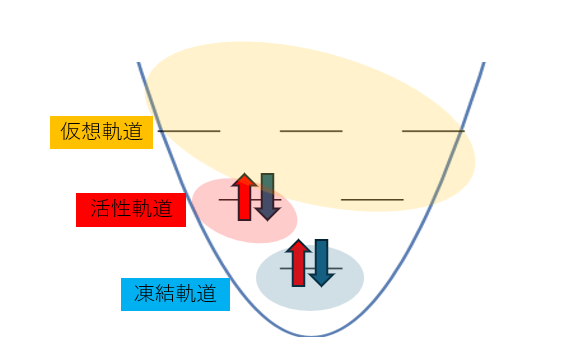
\includegraphics[width=0.75\linewidth]{imeges/kidou.png}
    \end{center}

  \end{frame}

    % --- 2.1.3 行列サイズの比較 ---
    \begin{frame}{2.3 近似手法と行列サイズの比較}
      スピン軌道k=12,電子数N=4, 
      \begin{itemize}
        \item Full CI: ${}_k C_N=495$
        \item SDCI:    $1 + {}_N C_1 \times {}_{k-N} C_1 + {}_N C_2 \times {}_{k-N} C_2=201$
        \item DCI:     $1 + {}_N C_2 {}_{k-N} C_2=169$
        \item 凍結軌道2個,活性軌道2個:${}_{k-2} C_{N-2}=45$ 
      \end{itemize}




      \end{frame}   

% --- 3章 序文スライド ---
\begin{frame}{第3章:CI解と一電子軌道の対称性}
  CI計算の品質は、用いる一電子基軌道の対称性に大きく依存する。
  計算時間削減の為に一電子軌道の数を制限すると,それだけ一電子軌道の対称性が
  多電子軌道の対称性につながることが考えられる.

  \vspace{1em}
  この章では、以下の視点から対称性と一電子基底の関係を議論する:
  \begin{itemize}
    \item UHFやGUHFで対称性がどのように壊れるか
    \item 対称性を保つ一電子軌道の構築方法(例:$\hat{L}_z$の固有状態)
    \item 対称性の壊れた軌道を使うとCI波動関数がどうなるか
  \end{itemize}
  
  \vspace{1em}
  最終的なCI解の美しさと対称性の保存には、一電子軌道の選定が極めて重要である。
  \end{frame}
  
  % --- 3.1 対称性の破れのメカニズム ---
  %--- 3.1.1 RHFの対称性保持 ---


  % --- 3.1.2 UHF/GUHFの対称性の破れ ---
  \begin{frame}{3.1 対称性の破れのメカニズム:UHFとGUHF}
    ハミルトニアン$\hat{H}$がある対称演算子(例:$\hat{L}_z$)と可換:
    \begin{align*}
    [\hat{H}, \hat{L}_z] = 0
    \end{align*}
    ならば、厳密な固有状態は$\hat{L}_z$の固有状態である。
    
    \vspace{1em}
    しかし、UHF/GUHFでは波動関数を\textbf{変分原理に従って最適化}するため、\textbf{軌道ごとに対称性が崩れた解を許す}:
    \begin{itemize}
      \item \textbf{UHF:} $\phi_i^{\alpha} \neq \phi_i^{\beta}$ により空間対称性が崩れ得る.
      \item \textbf{GUHF:} 混成スピン軌道により$\hat{S}_z$対称性も崩れ得る.
    \end{itemize}
    
    \vspace{1em}
    結果として、多体波動関数も$\hat{L}_z$, $\hat{S}_z$の固有状態でなくなることがある。
    これは、SCF解が\textbf{真の基底状態の対称性を自発的に破っている}ことに対応する。
    \end{frame}
  
% --- 3.2 CIの性質と一電子基底の選定 ---
\begin{frame}{3.2 CI解の対称性と一電子基底の選定}
  CI計算では、複数のスレーター行列の線形結合により、多体波動関数が構成される:
  \begin{align*}
  \hat{H} \Psi_{\text{CI}} = E_{\text{CI}} \Psi_{\text{CI}}
  \end{align*}
  
  \vspace{1em}
  CIは、理論的にはスピンや角運動量に関する固有状態を回復する力を持つが、
  それは\textbf{十分に対称性のあるスレーター行列基底がそろっている場合に限る}。
  
  \vspace{1em}
  しかし、\textbf{対称性が壊れた一電子軌道}を使うと:
  \begin{itemize}
    \item スレーター行列が$\hat{L}_z$や$\hat{S}_z$の固有状態でなくなる
    \item CI空間が対称性を持つ空間を張れなくなり、CI解も汚染される.
  \end{itemize}
  
  \vspace{1em}
  \textbf{対策:} 
  \begin{itemize}
    \item $\hat{L}_z$の固有状態から構成されるRHF軌道を使い、
  一電子基底に対称性を埋め込む。
    \item   自然軌道を使う.(勉強中)
  \end{itemize}
  \end{frame}
\end{document}